\subsection{CII Case Study}
The CII was formed by the Linux Foundation to support critical elements of the global information infrastructure by identifying and funding projects in need of assistance~\footnote{https://www.coreinfrastructure.org/faq}. The CII team has developed a census of open source projects in potential need of assistance~\footnote{https://www.coreinfrastructure.org/programs/census-project}, as well as a program for measuring and rewarding compliance with good security practice~\footnote{https://bestpractices.coreinfrastructure.org/}.

\subsubsection{Data selection}
\label{sec:cii_selection}
The CII census team has published the rationale behind their census and metrics ~\cite{wheeler2015open}, and has published their data and code on Github~\footnote{https://github.com/linuxfoundation/cii-census}. The 428 census records each contain data for one project deemed both important, and potentially at risk for security concerns, according to their criteria used by the CII team.

The project record contains descriptive data, e.g. project name and version, and security-relevant metrics, e.g. lines of code, contributor count, as well as an overall `risk index' based on the CII team's estimation of the importance of the metrics used to compute the index value.  Parallel to our translations of the CVSS metric score text to ordinal values, we translate the CII $fact\_activity$, $fact\_age$, $fact\_comments$, and $fact\_team\_size$ columns from text descriptions to ordinal values. We also parse the risk index components field to extract the ordinal ranks the CII team assigned each project for the risk index components: `Website points', `CVE Risk', `12 month contributors', `Popularity', `Language', and (network) `Exposure'. We now present our mapping of the CII metrics to our constructs.

\textbf{Asset Impact}
The CII package\_popularity field contains Debian package popularity contest~\footnote{http://popcon.debian.org/} results, a measure of the frequency of use of each package on each system, aggregated to the relative usage of the package within the Debian ecosystem. We reason that paclage popularity is proportional to our theorized `Number of Machines'  metric, and, so, should be modeled as a component of Asset Value.

\textbf{Software Risk}
We model total\_contributor\_count, Contributor Risk, and total\_code\_lines as components of Software Risk, on the rationale that multiple studies (e.g. ~\cite{camilo2015do,dashevskyi2016on}) have identified team size and code size as contributors to software vulnerability. The CII metrics direct\_network\_exposure and process\_network\_data, and potential\_privilege\_escalation are similar in concept to the CVSS Access metrics, and we, similarly, model them as components of Software Risk, theorizing that their values change based on design choices made by the software development team. We do not use the CII risk index measures, as they are composites, and we wish to examine the behavior of each of the index components.

\textbf{Adherence}
CII census data related to Adherence includes measurements of recent developer activity, and documentation effort. Developer activity is measured in the CII census data via a count of developers committing within the last year, twelve\_month\_contrib, and in terms of an ordinal categorical variable, fact\_activity, which we label TeamActivity. Documentation effort is measured in the CII census data via ordinal categorical variables in the risk index description for the amount and quality of comments, fact\_comments, which we label CodeComments, and by the presence of a website documenting the project, which we label WebsitePoints.

\textbf{Outcomes}
CII census data related to Outcomes includes a count of CVE vulnerabilities reported against the project since 2010. 

\textbf{Field choice notes}
The CII dataset contains a set of essentially co-linear fields, for example CVE Risk is translation of the CVE count since 2010 for the project into a categorical variable. We preferred counts to categorical values in initial field choices for the model.

\textbf{CII Data Exampes}
To illustrate how data is prepared for use in SEM estimation, Table \ref{tab:cii_data_examples} presents data from two example project, libexpat and procmail.  The table presents both the original data and the computed fields for each row, as used in SEM estimation.

% stargazer(t(ciicooked[1:2,]),style="asr")
% Table created by stargazer v.5.2 by Marek Hlavac, Harvard University. E-mail: hlavac at fas.harvard.edu
% Date and time: Wed, Mar 29, 2017 - 09:22:22
\begin{table}[!htbp] \centering 
		\caption{CII Original and Computed Data Examples}
		\label{tab:cii_data_examples}
	\begin{tabular}{@{\extracolsep{5pt}} crr} 
		\\[-1.8ex]\hline \\[-1.8ex] 
		Metric/Project & libexpat1 & procmail \\ 
		\hline \\[-1.8ex] 
		main\_language\_name & C & C \\ 
		CVE\_since\_2010 & 5 & 2 \\ 
		twelve\_month\_contributor\_count & 0 & 0 \\ 
		total\_contributor\_count & 10 &  4 \\ 
		total\_code\_lines & 22710 & 15536 \\ 
		package\_popularity & 174625 & 153379 \\ 
		direct\_network\_exposure & 0 & 1 \\ 
		process\_network\_data & 1 & 0 \\ 
		potential\_privilege\_escalation & 0 & 0 \\ 
		risk\_index & 13 & 13 \\ 
		CVE & 5 & 2 \\ 
		RiskIndex & 13 & 13 \\ 
		TeamActivity & 2 & 2 \\ 
		CodeAge & 4 & 4 \\ 
		CodeComments & 1 & 1 \\ 
		TeamSize & 0 & 0 \\ 
		WebsiteRisk & 0 & 0 \\ 
		CVERisk & 3 & 2 \\ 
		ContributorRisk & 5 & 5 \\ 
		PopularityRisk & 2 & 2 \\ 
		LanguageRisk & 2 & 2 \\ 
		ExposureRisk & 1 & 2 \\ 
		log12mcc & 0 & 0 \\ 
		logCVE2010 & 1.791759 & 1.098612 \\ 
		logCVECount & 1.791759 & 1.098612 \\ 
		KSLOC & 22.710 & 15.536 \\ 
		logKSLOC & 3.165897 & 2.805540 \\ 
		logSLOC & 10.03060 &  9.65098 \\ 
		logContributorCount & 2.302585 & 1.386294 \\ 
		logPackagePopularity & 12.07040 & 11.94067 \\ 
		\hline \\[-1.8ex] 
	\end{tabular} 
\end{table} 

\subsubsection{Data collection}

We retrieved the CII census data results file, current as of July 2016, from the project Github repository~\footnote{https://github.com/linuxfoundation/cii-census/blob/master/results.csv}. 

% stargazer(ciiraw)

% Table created by stargazer v.5.2 by Marek Hlavac, Harvard University. E-mail: hlavac at fas.harvard.edu
% Date and time: Sun, Feb 26, 2017 - 23:20:47
\begin{table*}[!htbp] \centering 
	\caption{} 
	\label{} 
	\begin{small}
	\begin{tabular}{@{\extracolsep{5pt}}lccccc} 
		\\[-1.8ex]\hline 
		\hline \\[-1.8ex] 
		Statistic & \multicolumn{1}{c}{N} & \multicolumn{1}{c}{Mean} & \multicolumn{1}{c}{St. Dev.} & \multicolumn{1}{c}{Min} & \multicolumn{1}{c}{Max} \\ 
		\hline \\[-1.8ex] 
		CVE\_since\_2010 & 428 & 7.262 & 26.142 & 0 & 422 \\ 
		twelve\_month\_contributor\_count & 346 & 98.965 & 491.693 & 0 & 3,768 \\ 
		total\_contributor\_count & 346 & 428.974 & 1,939.063 & 1 & 14,821 \\ 
		total\_code\_lines & 346 & 1,144,234.000 & 2,907,285.000 & 120 & 18,237,262 \\ 
		package\_popularity & 424 & 128,884.800 & 54,885.200 & 1 & 175,853 \\ 
		direct\_network\_exposure & 428 & 0.178 & 0.383 & 0 & 1 \\ 
		process\_network\_data & 428 & 0.152 & 0.359 & 0 & 1 \\ 
		potential\_privilege\_escalation & 428 & 0.058 & 0.235 & 0 & 1 \\ 
		risk\_index & 428 & 6.624 & 2.501 & 1 & 13 \\ 
		CVE & 428 & 7.262 & 26.142 & 0 & 422 \\ 
		RiskIndex & 428 & 6.624 & 2.501 & 1 & 13 \\ 
		TeamActivity & 428 & 1.509 & 0.988 & 0 & 3 \\ 
		CodeAge & 428 & 3.040 & 1.624 & 0 & 4 \\ 
		CodeComments & 428 & 2.231 & 1.773 & $-$1 & 5 \\ 
		TeamSize & 428 & 2.236 & 2.302 & $-$1 & 5 \\ 
		WebsiteRisk & 428 & 0.131 & 0.338 & 0 & 1 \\ 
		CVERisk & 428 & 1.044 & 1.266 & 0 & 3 \\ 
		ContributorRisk & 428 & 1.722 & 1.981 & 0 & 5 \\ 
		PopularityRisk & 428 & 1.808 & 0.494 & 0 & 2 \\ 
		LanguageRisk & 428 & 1.360 & 0.934 & 0 & 2 \\ 
		ExposureRisk & 428 & 0.558 & 0.777 & 0 & 2 \\ 
		DataRisk & 428 & 0.000 & 0.000 & 0 & 0 \\ 
		\hline \\[-1.8ex] 
	\end{tabular} 
	\end{small}
\end{table*}

We examined the variable variances, and log transformed the largest of them: total\_code\_lines, total\_contributor\_count, and package\_popularity.

We checked for collinearity between measurement variables. We eliminated twelve\_month\_ contributor\_count, and TeamSize based on their collinearity with total\_contributor\_count. We eliminated ExposureRisk based on its collinearity with direct\_network\_exposure, and PopularityRisk based on its collinearity with package\_popularity.

\subsubsection{Estimation}
Combining the structural and measurement models we have defined with the metric data collected from the CII census, we have the initial model definition, expressed in lavaan syntax, as follows:

\begin{align*}
SoftwareRisk =\sim  total\_contributor\_count + ContributorRisk \\ + total\_code\_lines 
+ LanguageRisk + direct\_network\_exposure\\
 + process\_network\_data 
+ potential\_privilege\_escalation + CodeAge \\
AssetImpact =\sim package\_popularity \\
Outcomes =\sim  logCVECount \\
Adherence =\sim  TeamActivity + CodeComments + 
	twelve\_month\_contributor\_count\\  + WebsiteRisk  \\
Outcomes \sim SoftwareRisk + AssetImpact \\
SoftwareRisk \sim  Adherence \\
AssetImpact \sim\sim  Adherence\\
SoftwareRisk \sim\sim 0*AssetImpact\\
Adherence \sim\sim 0*Outcomes\\
\end{align*}

\subsubsection{Model Fit}
The initial model did not converge, after 678 iterations over the CII dataset. We describe the steps we took to respecify the model in the next section.
 
\subsubsection{Re-specification}
Given that the initial model did not converge, we took the following steps to revise the model.

To assess fit difficulties in the measurement model, per Loehlin~\cite{loehlin1986latent}, we fit the data to a model in which all latent variables are correlated with each other, which has the effect of removing structural model fit concerns, allowing measurement model fit to be examined. In this step, the model converged, but yielded very poor fit (CFI 0.076, NFI -.152, RMSEA 0.214, SRMR 0.167), revealing that the initial set of measurement variables is poorly matched to the structural model.  

Given that the fit results did not meet standard fit criteria thresholds, we consider a set of alternative measurement models, guided by our theoretical justification for each choice of measurement variable. We conduct an exploratory analysis, retaining the structural model, and altering the measurement model one measurement variable at a time. For each measurement variable in the Software Risk and Asset Impact constructs, we drop a single measurement variable and re-estimate the model fit. 

None of the re-specified models met all of the fit criteria thresholds, however several met at least one threshold. We present the closest fitting model in the Respecified CII column of Table \ref{tab:results_fit_all}. We present the parameter estimates for the Respecified CII model in the results, and discuss the implications in Section \ref{sec:case_cii_discussion}.

\subsubsection{Reporting Results}
\label{sec:case_cii_results}

Table \ref{tab:results_fit_all} presents the fit measure results in the Respecified CII model column. We report the estimated parameter values in \ref{tab:results_cii}.

\begin{table}
	\begin{center}	
		\caption{CII Respecified Model Results}
		\label{tab:results_cii}
		\begin{tabular}{l|rrrr}
			\\[-1.8ex]\hline 
			\hline \\[-1.8ex] 
			\textit{Latent Variables}:  & & & & \\  
			$\sim$ Measured variables& Estimate & Std.Err & z$-$value & $P(>|z|)$ \\
			\hline \\[-1.8ex]
			$SoftwareRisk =\sim$  & & & & \\  
		    logContrbtrCount  &  1.000   & &  &   \\           
		    ContributorRisk  &  $-$0.909  &  0.063 & $-$14.350 &   0.000\\		
		    logSLOC        &   0.781  &  0.071  & 10.947  &  0.000\\
		    drct\_ntwrk\_xps &   0.025  &  0.012  &  2.182  &  0.029\\
		    prcss\_ntwrk\_dt &  -0.007  &  0.011  & -0.625  &  0.532\\
		    ptntl\_prvlg\_sc &  -0.004  &  0.007  & -0.522  &  0.602\\
		    CodeAge        &   0.201  &  0.021  &  9.360  &  0.000\\	
			$AssetValue =\sim$     & & & & \\                                    
			logPackagePopularity   & 1.000     & & & \\                       
			$Outcomes =\sim$    & & & & \\                                     
			logCVECount     &  1.000  & & & \\                          
			$Adherence =\sim$   & & & & \\                                      
			Team Activity    &     1.000        & & & \\      
			CodeComments  &   $-$1.235 &   2.449 &  -0.504 &   0.614\\
			WebsiteRisk   &   -0.069  &  0.104  & -0.664 &   0.507\\              
			Regressions:  & & & & \\  
			%& Estimate & Std.Err & z$-$value & $P(>|z|)$ \\
			$Outcomes \sim$         & & & & \\                                     
			SoftwareRisk   &  0.200 &   0.040 & 4.999 &   0.000 \\
			AssetImpact     &   $-$0.137  &  0.051  &  $-$2.707 &   0.007\\
			$SoftwareRisk \sim$        & & & & \\                                  
			Adherence     &    -0.437 &   0.799  &  $-$0.546 &   0.585\\
			Covariances:  & & & & \\  
			%& Estimate & Std.Err & z$-$value & $P(>|z|)$ \\
			$AssetValue \sim\sim$          & & & & \\                                 
			Adherence      &  0.007  &  0.035 &  0.199 &   0.842\\
		\end{tabular}
	\end{center}
\end{table}

As mentioned above, the Respecified CII model had mixed results for traditional fit criteria, as measured by the fit indexes, so the hypothesis tests for the model should be viewed with caution. 

Interpreting the parameter estimates in terms of our hypothesized construct relationships, we have the following:
\begin{itemize}
	\item  Asset Impact is negatively associated (-0.14) with Security Outcomes, contrary to what we hypothesized.
	\item Software Risk is positively associated (0.28) with Security Outcomes, as hypothesized. 
	\item Practice Adherence is negatively associated (-0.44) with Software Risk,  
	as we hypothesized. 
\end{itemize}	
Asset Impact - Security Outcomes and Software Risk - Security Outcomes were statistically significant, Practice Adherence - Software Risk was not statistically significant. 

We present the standardized parameter estimates, and the residuals, in the context of the full structural and measurement models in Figure \ref{fig:cii_model_respecified_estimates}. Circles represent the latent variables/constructs of the structural model. Squares represent the measurement variables of the measurement model. Lines indicate relationships between variables.

\begin{figure*}
	\centering
	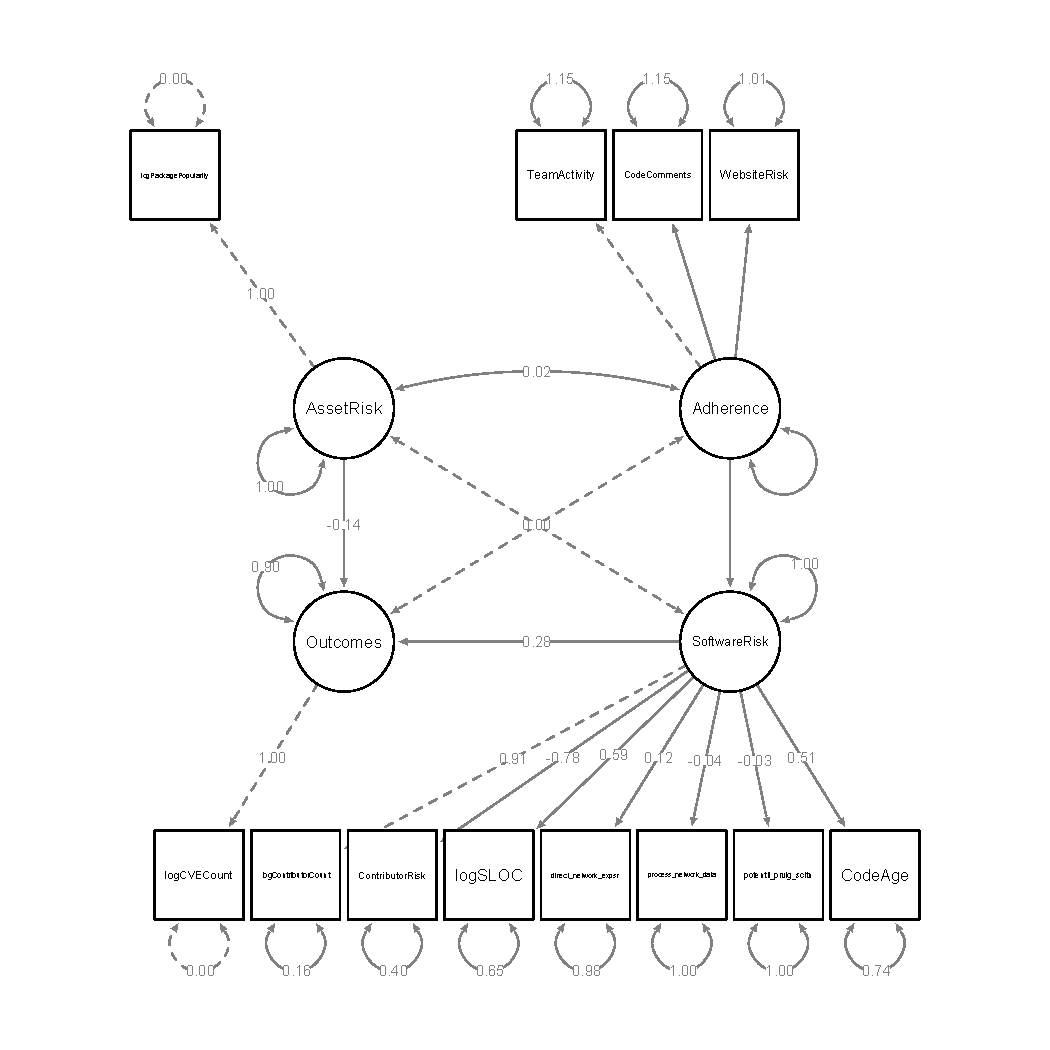
\includegraphics[width=.6\textwidth]{CII_Respecified_SEM_Model.pdf}
	\caption{Respecified CII Model}
	\label{fig:cii_model_respecified_estimates}
\end{figure*}
 